% =====================================================================
% 6.2 Regimes de amortecimento
% =====================================================================
\subsection{Regimes de amortecimento}

A Tabela~\ref{tab:regimes} repete os três métodos com \(h=2~\mu\mathrm{s}\) nos três regimes. O RK4 mantém o erro máximo da corrente entre \(10^{-10}\) e \(10^{-8}\)~A. O caso sobreamortecido tem o maior erro do RK4 porque o seu polo mais rápido, \(\lambda\approx -4{,}79\times 10^{4}~\mathrm{s}^{-1}\), exige mais do passo: \(h|\lambda|\approx 0{,}096\). Mesmo assim, esse erro é desprezível diante de correntes de miliampères. A Figura~\ref{fig:regimes} mostra que a curva do RK4 e a curva exata se confundem nos três regimes.

\begin{table}[htbp]
\centering
\caption{Erro máximo da corrente, em ampères, com \(h=2~\mu\mathrm{s}\) e \(t_f=5~\mathrm{ms}\), nos três regimes.}
\label{tab:regimes}
\small
\begin{tabular}{@{}lrrr@{}}
\toprule
Regime & Euler & Euler melhorado & RK4 \\
\midrule
Subamortecido, \(R=20~\Omega\) & \(1{,}95\times 10^{-3}\) & \(1{,}23\times 10^{-5}\) & \(2{,}46\times 10^{-10}\) \\
Crítico, \(R=200~\Omega\) & \(2{,}34\times 10^{-4}\) & \(2{,}72\times 10^{-6}\) & \(1{,}03\times 10^{-10}\) \\
Sobreamortecido, \(R=500~\Omega\) & \(2{,}00\times 10^{-4}\) & \(6{,}60\times 10^{-6}\) & \(3{,}05\times 10^{-9}\) \\
\bottomrule
\end{tabular}
\fonte{Elaborado pelos autores (2026).}
\end{table}

\begin{figure}[htbp]
\centering
\caption{Corrente do degrau nos três regimes. A curva exata e o RK4 com \(h=2~\mu\mathrm{s}\) aparecem sobrepostos.}
\label{fig:regimes}
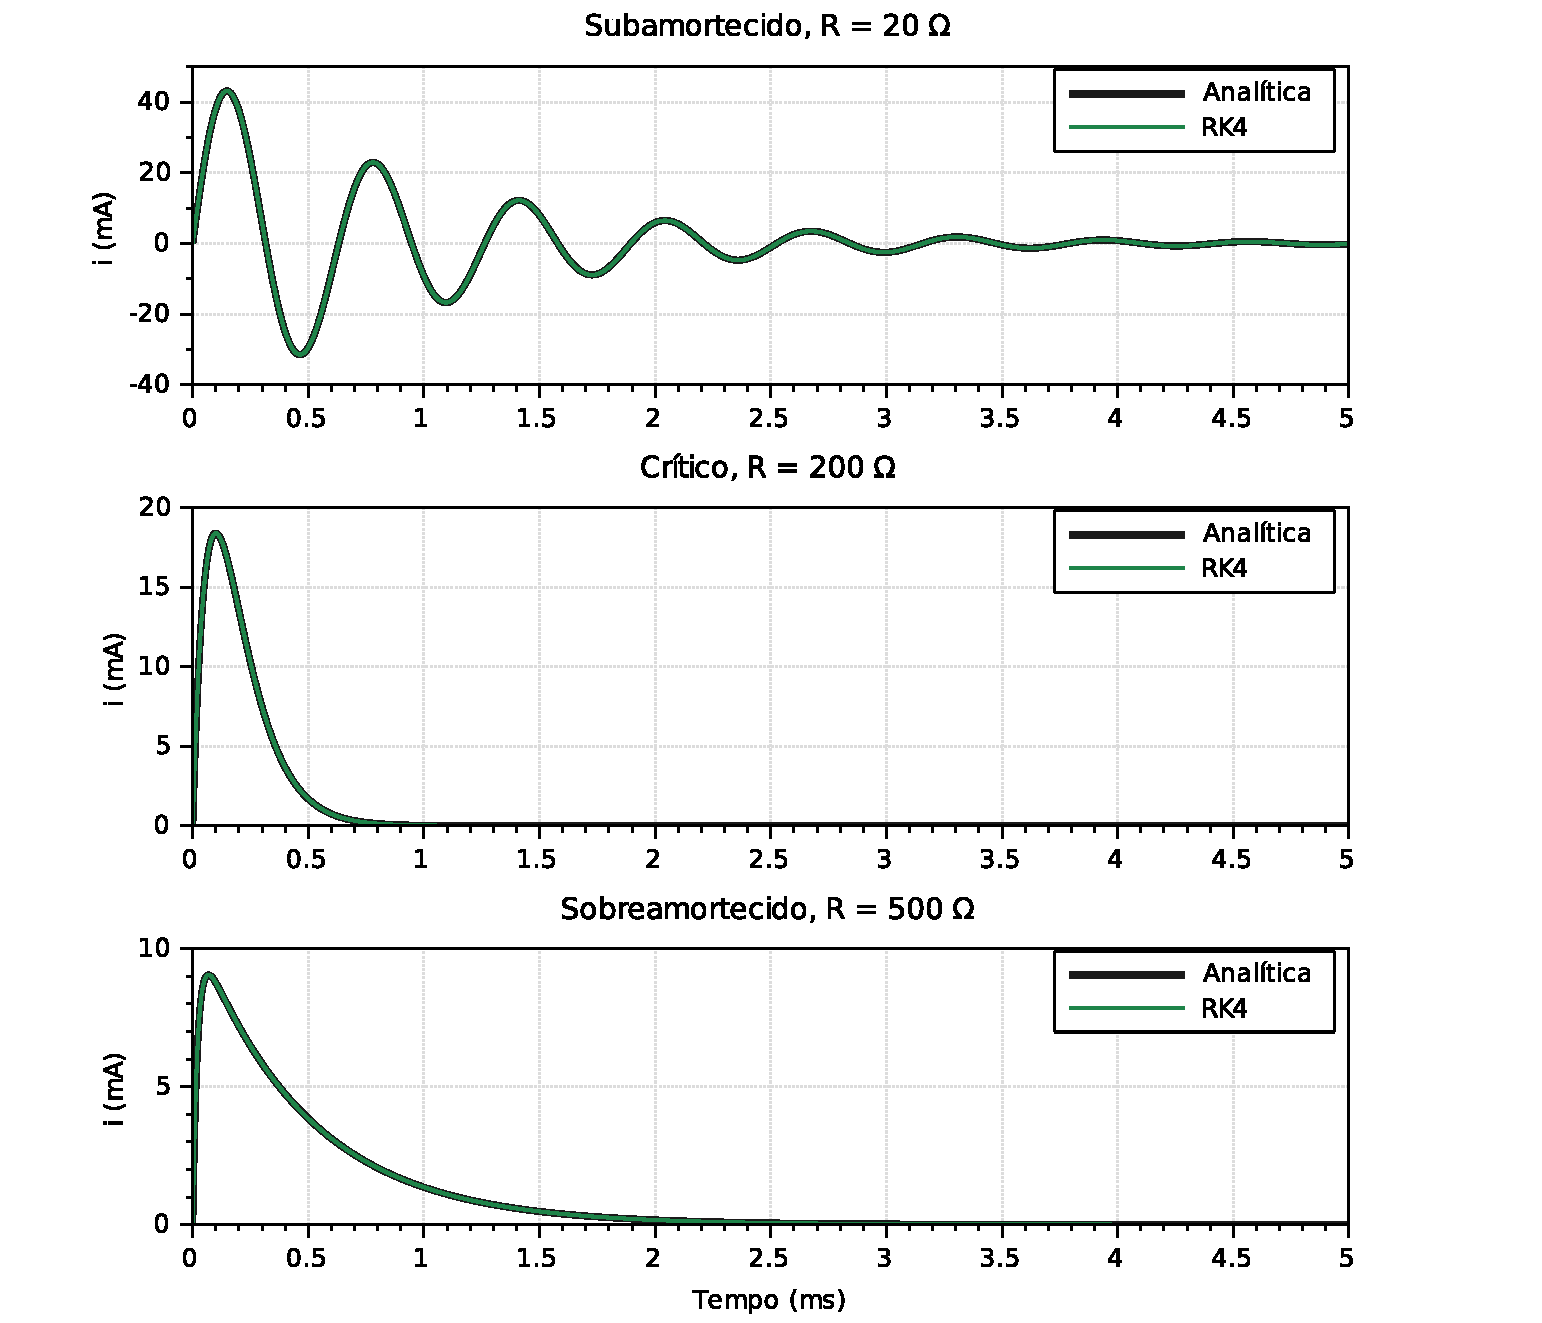
\includegraphics[width=0.94\textwidth]{regimes.pdf}
\fonte{Elaborado pelos autores (2026).}
\end{figure}

O resultado mostra que os métodos não dependem do regime para funcionar. O que muda de um regime para outro é o polo mais rápido, e é ele que limita o passo.
